\documentclass[letter]{article}

\usepackage[margin=1.1in]{geometry}
\usepackage[english]{babel}
\usepackage[utf8]{inputenc}
\usepackage{amsmath}
\usepackage{graphicx}
\usepackage{lipsum}
\usepackage{setspace}
\usepackage[bottom]{footmisc}
\usepackage[colorinlistoftodos]{todonotes}
\usepackage{pdfpages}

\newcommand\blfootnote[1]{%
	\begingroup
	\renewcommand\thefootnote{}\footnote{#1}%
	\addtocounter{footnote}{-1}%
	\endgroup
}



\begin{document}
\begin{figure}[t]
\centering

\includegraphics[width=0.4\textwidth]{img/dropLogo.png}
\end{figure}
\title{Physics Honors Project Defense - DROP: A multi-point flood monitoring system}

\author{Jacob Dice - William Jewell College}


\date{\today}
\maketitle



\begin{abstract}
\setstretch{1.5}

Natural disasters are occurring at an increasing frequency. One of these natural disasters is inland flooding. Excessive rainfalls from atypical storm systems or hurricanes can cause extreme flooding conditions. This is evident with recent and irregular storm systems, including hurricane Irma, hurricane Harvey, and hurricane Michael, just to name a few. During and after such intense rainfalls, roadways are flooded and homes are underwater. This honors project is centered around creating an urban flood monitoring device that provides three primary benefits: First, officials can monitor floods and determine water depths as the floodwater propagates and combines with run-off through the city. With precise monitoring, officials will be able to know the best way to navigate through an urban area after a flood. Second, flood water movement is difficult to estimate and many models are made with data collected after the flood, based on water marks on buildings. Having accurate real-time flood data will provide data to enhance our current models. Finally, our insurance agencies are basing premiums off metrics such as the `hundred year flood line'. This sensor will provide much better data for statistical analysis to update historical models.  
\end{abstract}
\blfootnote{I would like to thank Dr. Baker as my advisor for this project and all of the Honors Project Committee members for their guidance throughout the development of this sensor. In addition, I would like to thank Dr. McCoy, Dr. Bots, and Dr. Bunton for serving on my Defense Committee.}

\pagebreak

\tableofcontents

\pagebreak
\section{Introduction and Motivation}
\label{sec:introduction}
\setstretch{1.5}

Inland flooding is an immense safety concern for individuals in certain geographic regions. With excess rainfall, floodwater can collect due to runoff and inadequate city drainage infrastructure. As natural disasters occur at an increasing rate, it is imperative that we provide adequate data to our citizens to make safe decisions, to our rescue crews to safely and effectively rescue individuals in danger, and to our city officials to design adequate drainage infrastructure. With granular sensor data, DROP can provide rescue crews pertinent information during their rescue operations, create better flood models, and update statistical estimations of potential flood damages.

To generate flood data, I have created DROP. DROP is an electrical circuit that monitors floods and will deployed at multiple locations in a city. At each location, there will be a combination of a control board and a water depth sensor that will wirelessly transmit the water depth data to an online web server. Numerous water depth data points across a city, in conjunction with an accurate topographical map, can be used to interpolate the areas with flood water and will allow city officials to track flood waters as it propagates through a city. DROP will provide public utility in exceptional storm systems such as hurricane Harvey, or the other recent and extreme natural disasters we have experienced. Below I give more detail on the motivation for this project and how DROP improves safety. 
\subsection{Public Safety}

One of the motivations for DROP is to allow the general public to be more informed of flood conditions and make better decisions in flood prone weather conditions. According to The Weather Channel, the trend of intense flooding, ``will likely continue as climate change increases the rick of heavy rainfall'' \cite{floodDeaths}. To quantify this, they have calculated the number of days with extremely heavy precipitation. In both wet and dry locations, the number of days has increased 1\% to 2\% each decade over the last 60 years. Moreover, the annual number of deaths has increased. See figure \ref{fig:floodDeaths} for the average number of deaths per year. 
\begin{figure}[ht]
\centering
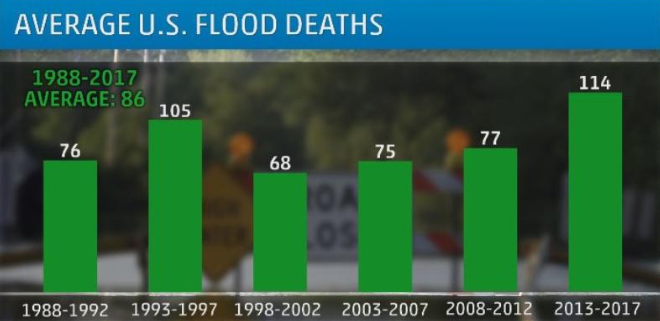
\includegraphics[width=.6\textwidth]{img/floodDeaths.png}
\caption{\label{fig:floodDeaths}The average number of deaths per year, averaged over 5 year periods. \cite{floodDeaths}.}
\end{figure}

While we cannot directly control rainfall, if we can provide our citizens with pertinent information during floods and provide our rescue crews with water depth data during floods, we should be able to prevent the loss of life during these natural disasters. Granular floodwater data will aid in these efforts. 

\subsection{Economic Impact}
In addition to loss of life, there are extensive economic impacts caused by flooding. As climate change leads to an increased frequency of flooding, many homes, business, and farms are damaged. An article on The Balance claims that there has been \$260 Billion dollars in damages between 1980 and 2013 \cite{economicImpact}. In response to the devastating impacts to people and businesses, the United States Government created the National Flood Insurance Program (NFIP) in 2004. This program allows private and public infrastructure to be affordably insured against flooding. However, since 2004, NFIP has ``accumulated \$39.4 billion in debt'' \cite{economicImpact}. Essentially, the premiums charged by NFIP have not been sufficient to cover claims on insurance policies. The same article by The Balance highlights that, "many homes in recent floods did not have flood insurance because they were outside the 100-year floodplain" \cite{economicImpact}. I would like to attribute this deficit and lack of insurance to inadequately understanding the risks of flood zones. Theoretically, the 100-year floodplain defines geographical areas that are prone to flooding once every 100 years (1\% probability of flooding annually). During Hurricane Harvey, 75\% of the homes damaged were not even within a 100-year floodplain area \cite{economicImpact}. This raises the question, are 100-year floodplains accurate? If not, we need to find other proxies to base our insurance premiums on and to appropriately educate homeowners of the true flooding risks. The granular sensor data that DROP provides will help to answer these types of questions. 

\subsection{Uncertainty of Flooding Conditions}

The difficulty predicting floods is partially caused by the numerous causes of inland floods. Since we cannot predict flood probability, we cannot accurately inform the public or inform our economic and insurance models. Figure \ref{fig:floodCauses} shows a few of the leading causes of inland floods. 

\begin{figure}[ht]
	\centering
	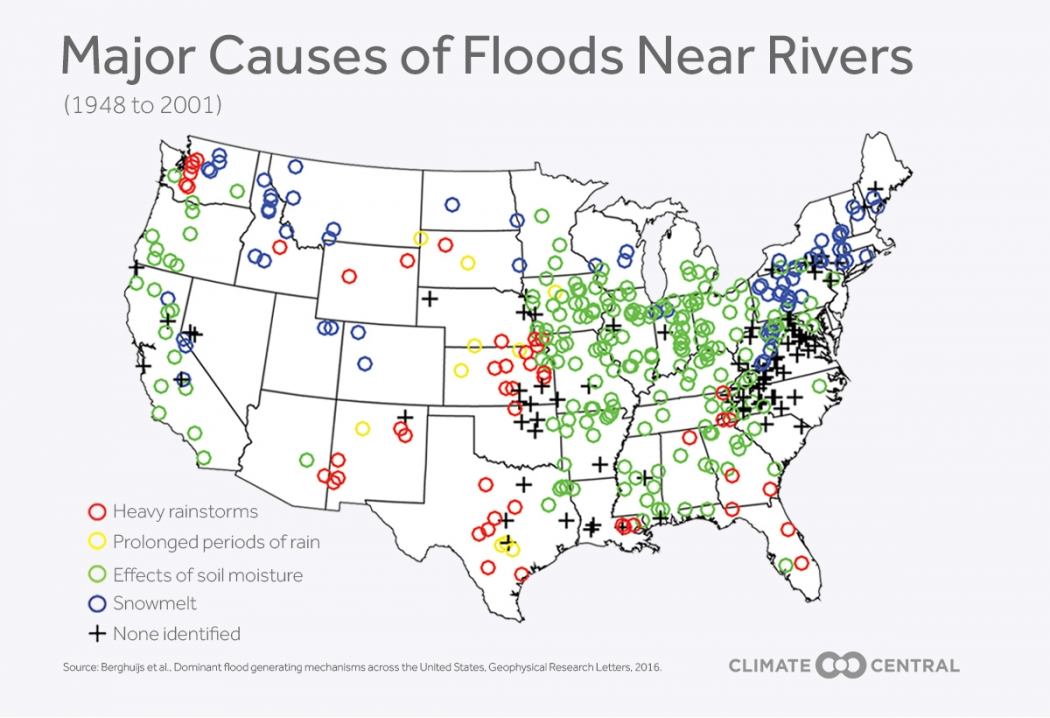
\includegraphics[width=.8\textwidth]{img/causesOfFlooding.jpg}
	\caption{\label{fig:floodCauses} This figure shows the primary cause of floods geographically. \cite{floodDays}.}
\end{figure}

As the figure shows, the causes of flooding are extremely variable. The probability of flooding can be effected by heavy rainstorms, prolonged periods of rain, soil moisture, and snowmelt \cite{floodDays}. Moreover, in a developed area, flash flooding can be greatly impacted by the hardscapes on the ground. Watershed behaves differently on pavement, dirt, rock, etc. In a city where a large percentage of the ground is a hardscape (sidewalks, roads, roofs, or any impermeable surface), watershed relies on robust city drainage infrastructure. The reason I comment on the numerous causes of floods is because it is difficult to create a model that predicts floods without knowing how a specific geographical area responds to rainfall. The sensor data from DROP will provide this granular data to create accurate flood models. 

\subsection{Market Research}
When starting this project, I wanted to make sure I was designing a product for a real problem in a given geographical area. To research potential markets for DROP, I contacted many city engineers to discuss the challenges they face regarding public safety and city infrastructure. This process was very enlightening because I learned the concerns and thought processes of the individuals in charge of flood engineering for a city. A particularly enlightening call I had was with a city engineer in Florida. The call was primarily about the nature of flooding in coastal areas of Florida. I learned that, although coastal areas, such as Florida, flood frequently, the relatively flat terrain and proximity to sea level mean that their ``floods'' are not what a typical mid-western flood looks like. As the city engineer described, their flood might be a foot high, but after that it drains to the ocean quickly enough that they do not have serious runoff issues. This was very useful information because it provided a perspective that I had not considered with my background growing up in Kansas City. This insight shaped the potential markets for this flood monitoring sensor. Although floods are frequent in Florida, the geography is generally not conducive for deep floodwaters. Instead, I need to design a sensor that will be deployed in a Midwest area with elevation variation causing potential for runoff.

\section{Control Board Sensor Design}
\label{sec:control board}
Through my market research, I identified the main problems and geographies that are affected by flooding. The development of DROP was greatly impacted by this research, and is evident in the design iterations.

I have segmented the flood sensor into two main components. The control board and the water sensor. The control board is the device that will record and transmit the water depth information. To record the water depth, it is attached to a physical electrode board (which I call the water sensor). In the following section, I will describe the three primary iterations of the control board. 

\subsection{DROP Control Board Version 1}
 The initial idea and design was seeded from a Global Design Competition called Invent for the Planet (IFTP), held at Wichita State University in the spring of 2018. A group of Jewell UIF students attended this event and ideated about this type of monitoring system. During this competition, I fabricated the first control board. The initial design from IFTP was a very rough prototype, only showing proof of concept. It was a hardwired sensor that attached to my computer and used bare wire as the conductor for the water depth sensor. Figure \ref{fig:v1Board} shows an image of the first control board.
 
\begin{figure}[ht]
 	\centering
 	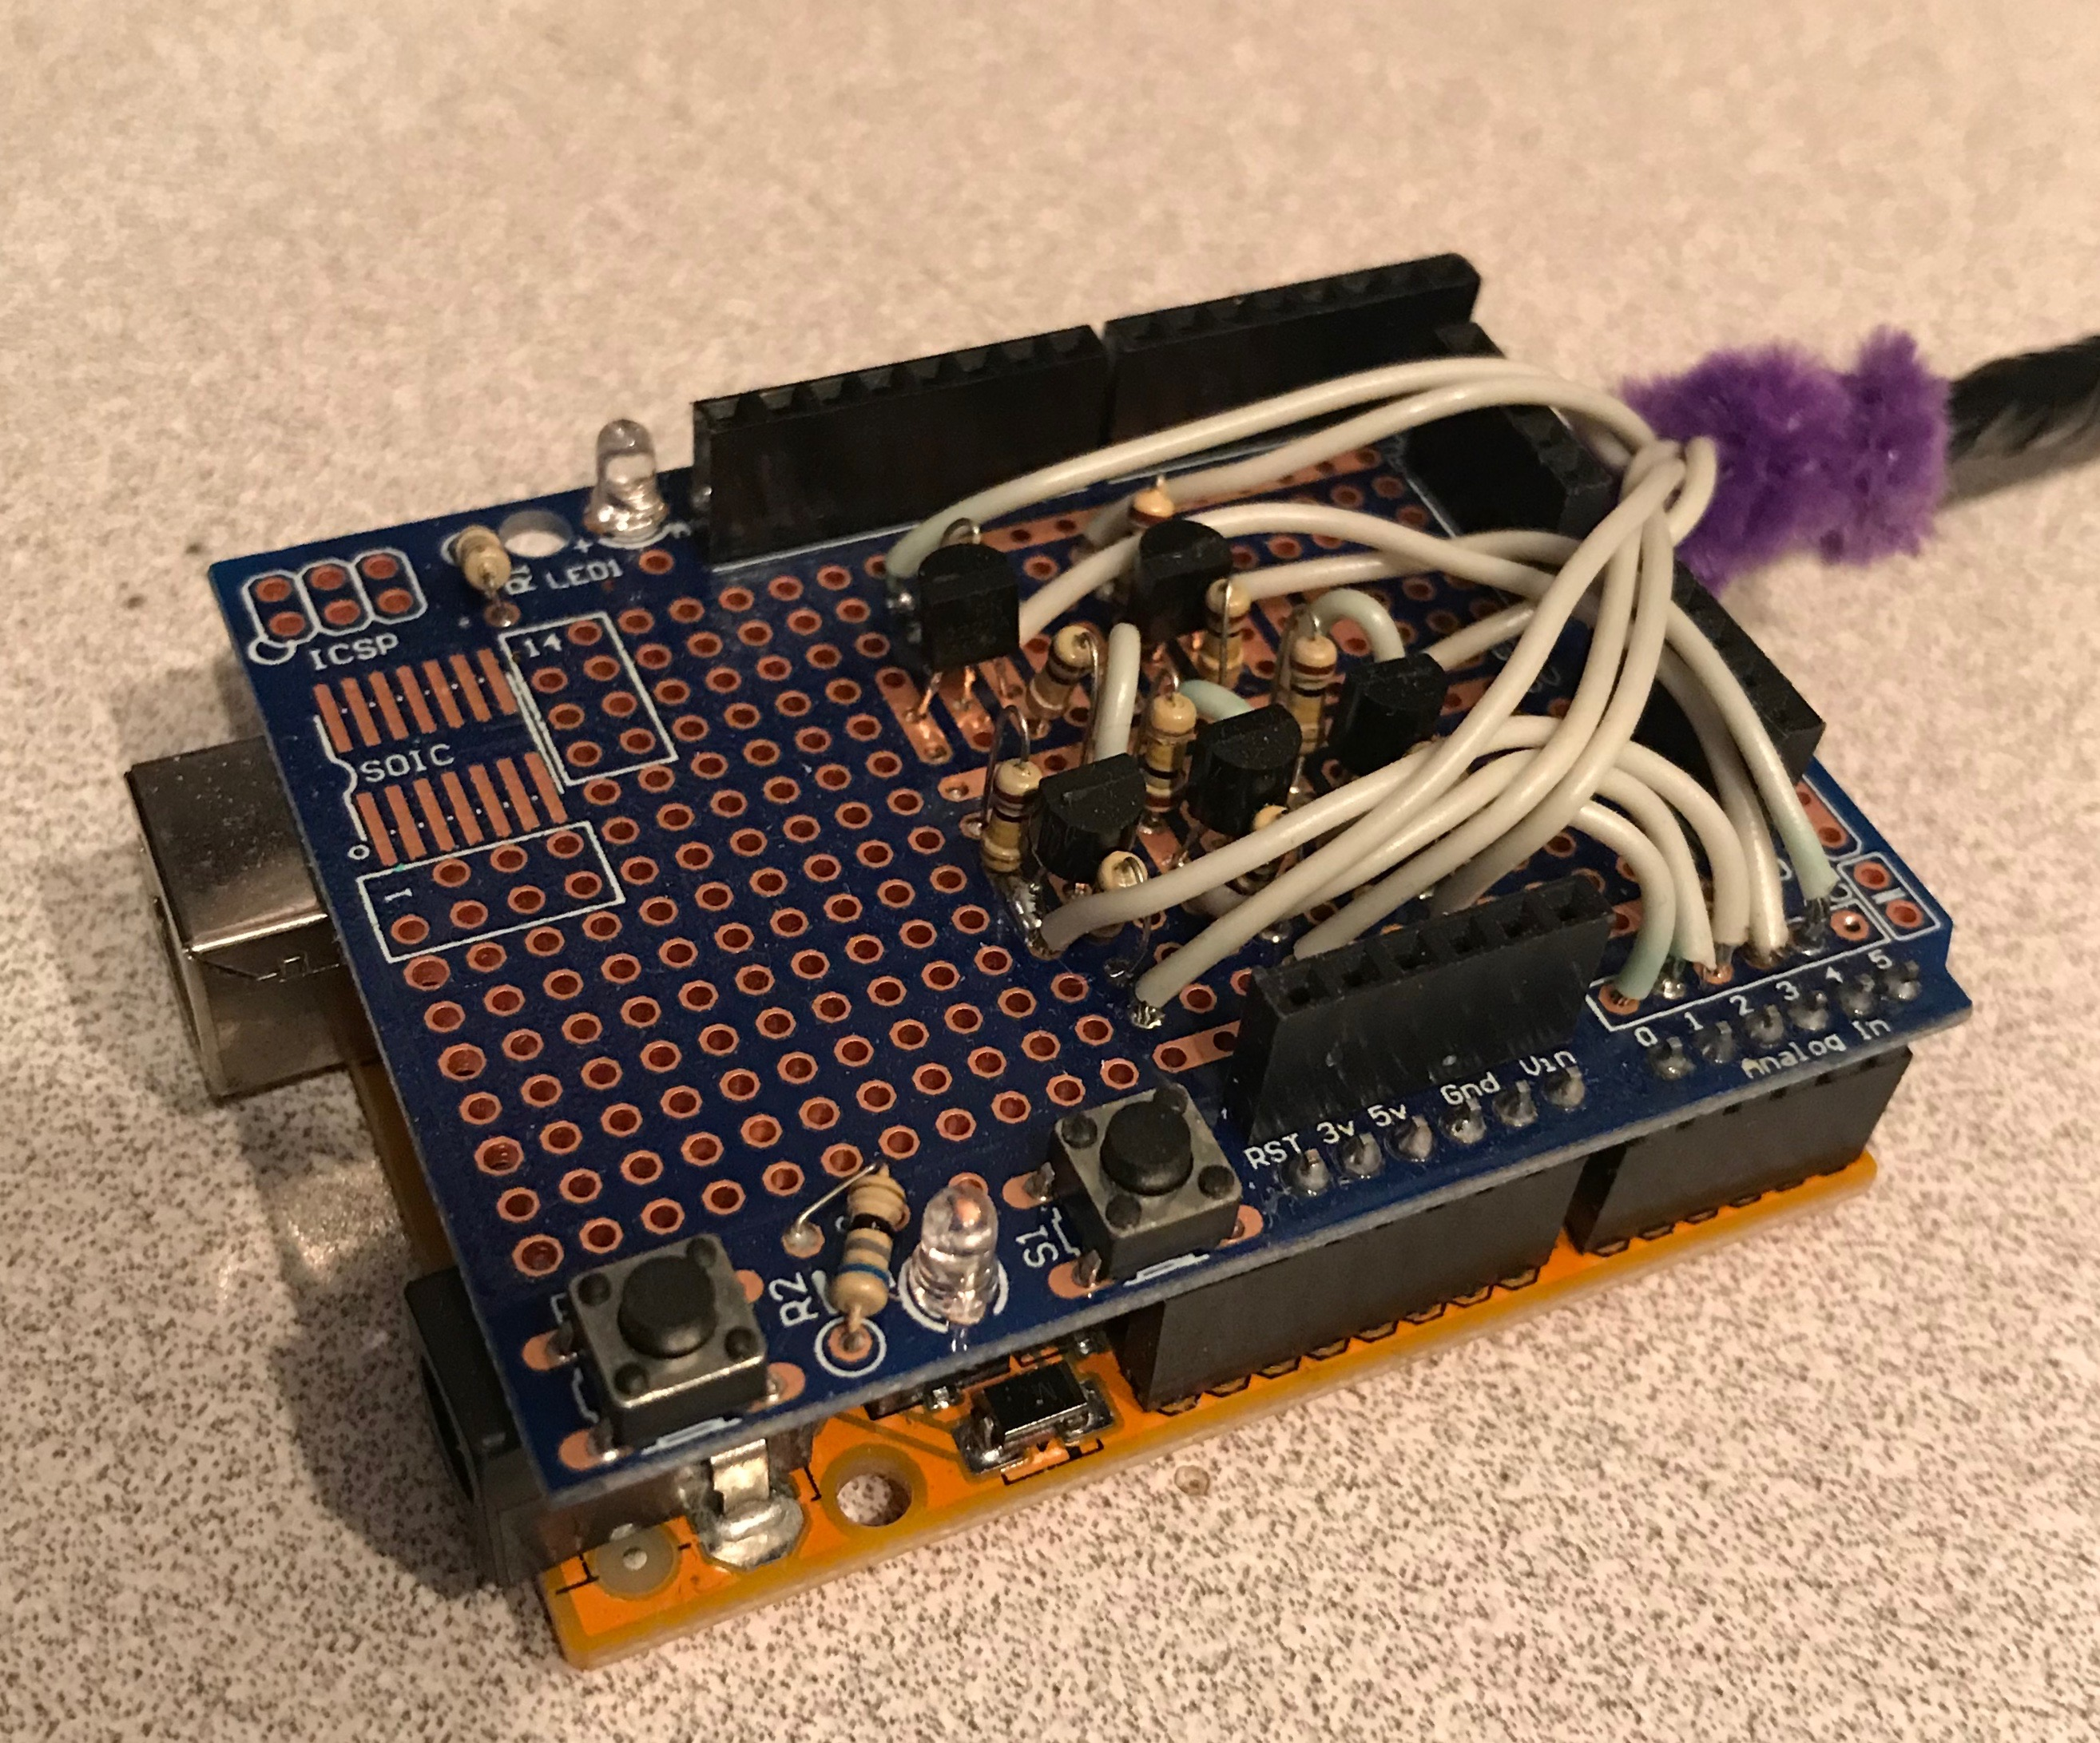
\includegraphics[width=.5\textwidth]{img/v1_ControlBoard.jpg}
 	\caption{\label{fig:v1Board} This figure shows the version 1 control board.}
\end{figure}

\begin{figure}[ht]
	\centering
	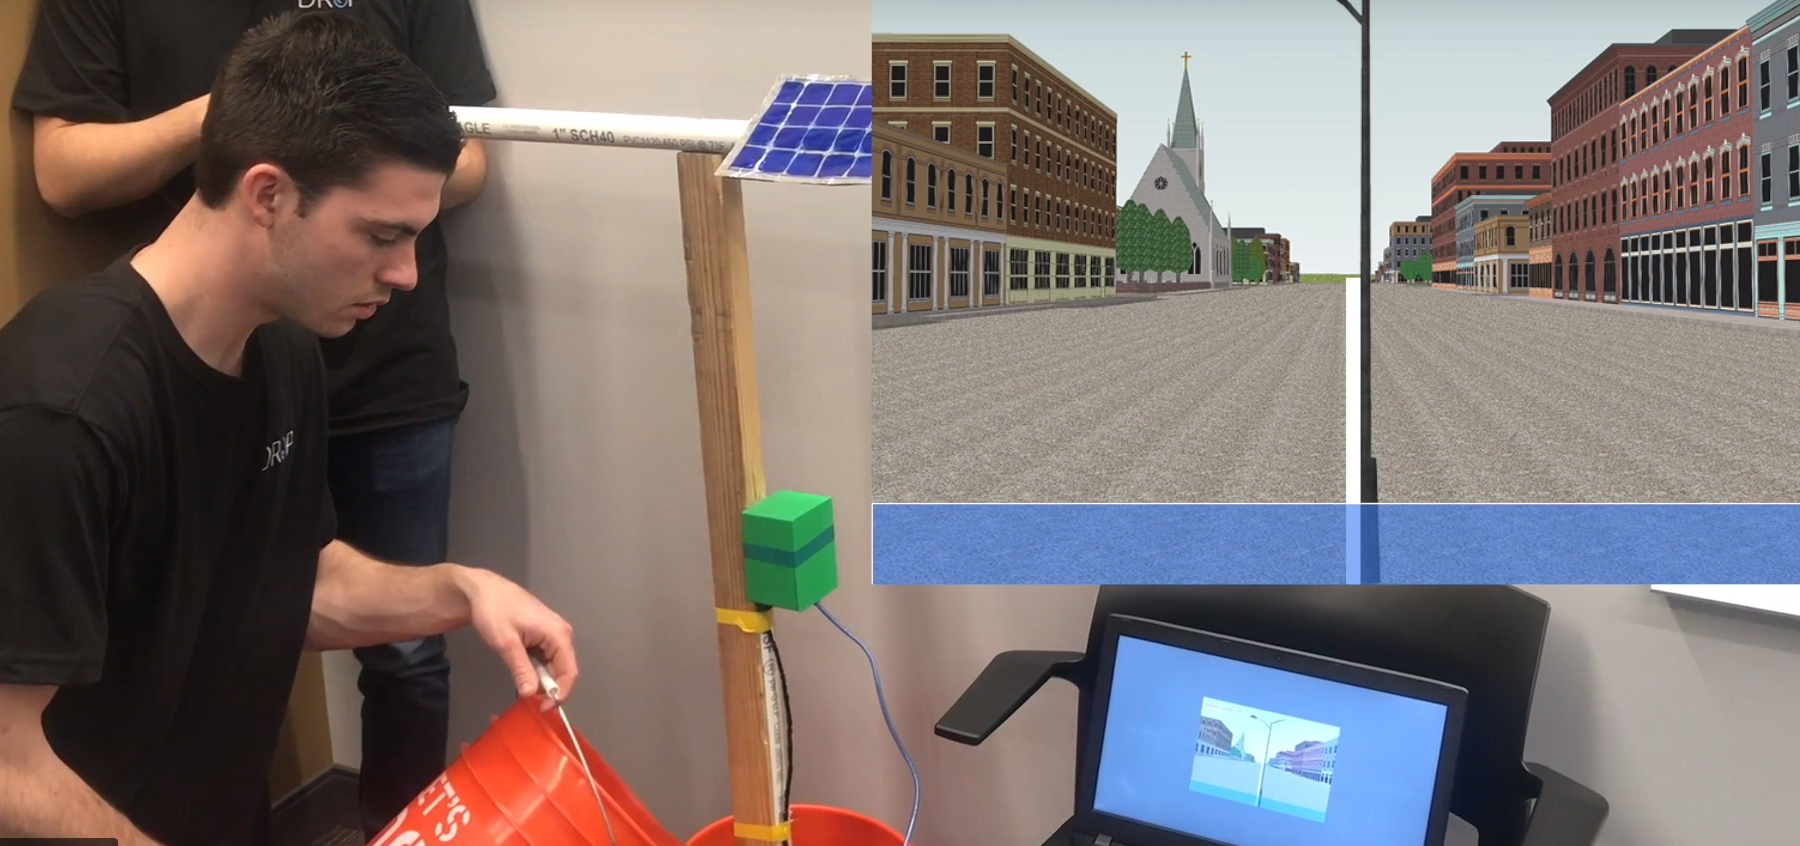
\includegraphics[width=.7\textwidth]{img/v1_WaterDepth.PNG}
	\caption{\label{fig:v1WaterDepth} This figure shows the version 1 water depth sensor and computer program that plots the depth.}
\end{figure}
This prototype implemented the bare minimum for a proof of concept. It included an Arduino Uno with five transistor amplifiers that were used to measure 5 discrete water levels. The water sensor was soldered to this board and consisted of a few wires hot glued to a PVC pipe. I wrote a program to take this data and plot the flood level on a computer. The water sensor and computer program are shown in Figure \ref{fig:v1WaterDepth}. While the first iteration showed proof of concept that an electrode-style water depth meter would function as expected, it needed significant work to create a viable and scalable product. Version 2 and Version 3 of the control board add useful features and make the product viable for mass manufacturing. 
 
\subsection{DROP Control Board Version 2}
Version 2 is the intermediate version of the DROP control board. After deciding to pursue this project as my honors project, I began to research design considerations and component selection that would be robust enough to implement in a production run of this sensor. In this iteration, I implemented features that I learned would be useful from my market research. Figure \ref{fig:v2_controlBoard} shows the final version 2 prototype. I soldered it together on a protoboard with many off the shelf components. 

\begin{figure}[ht]
	\centering
	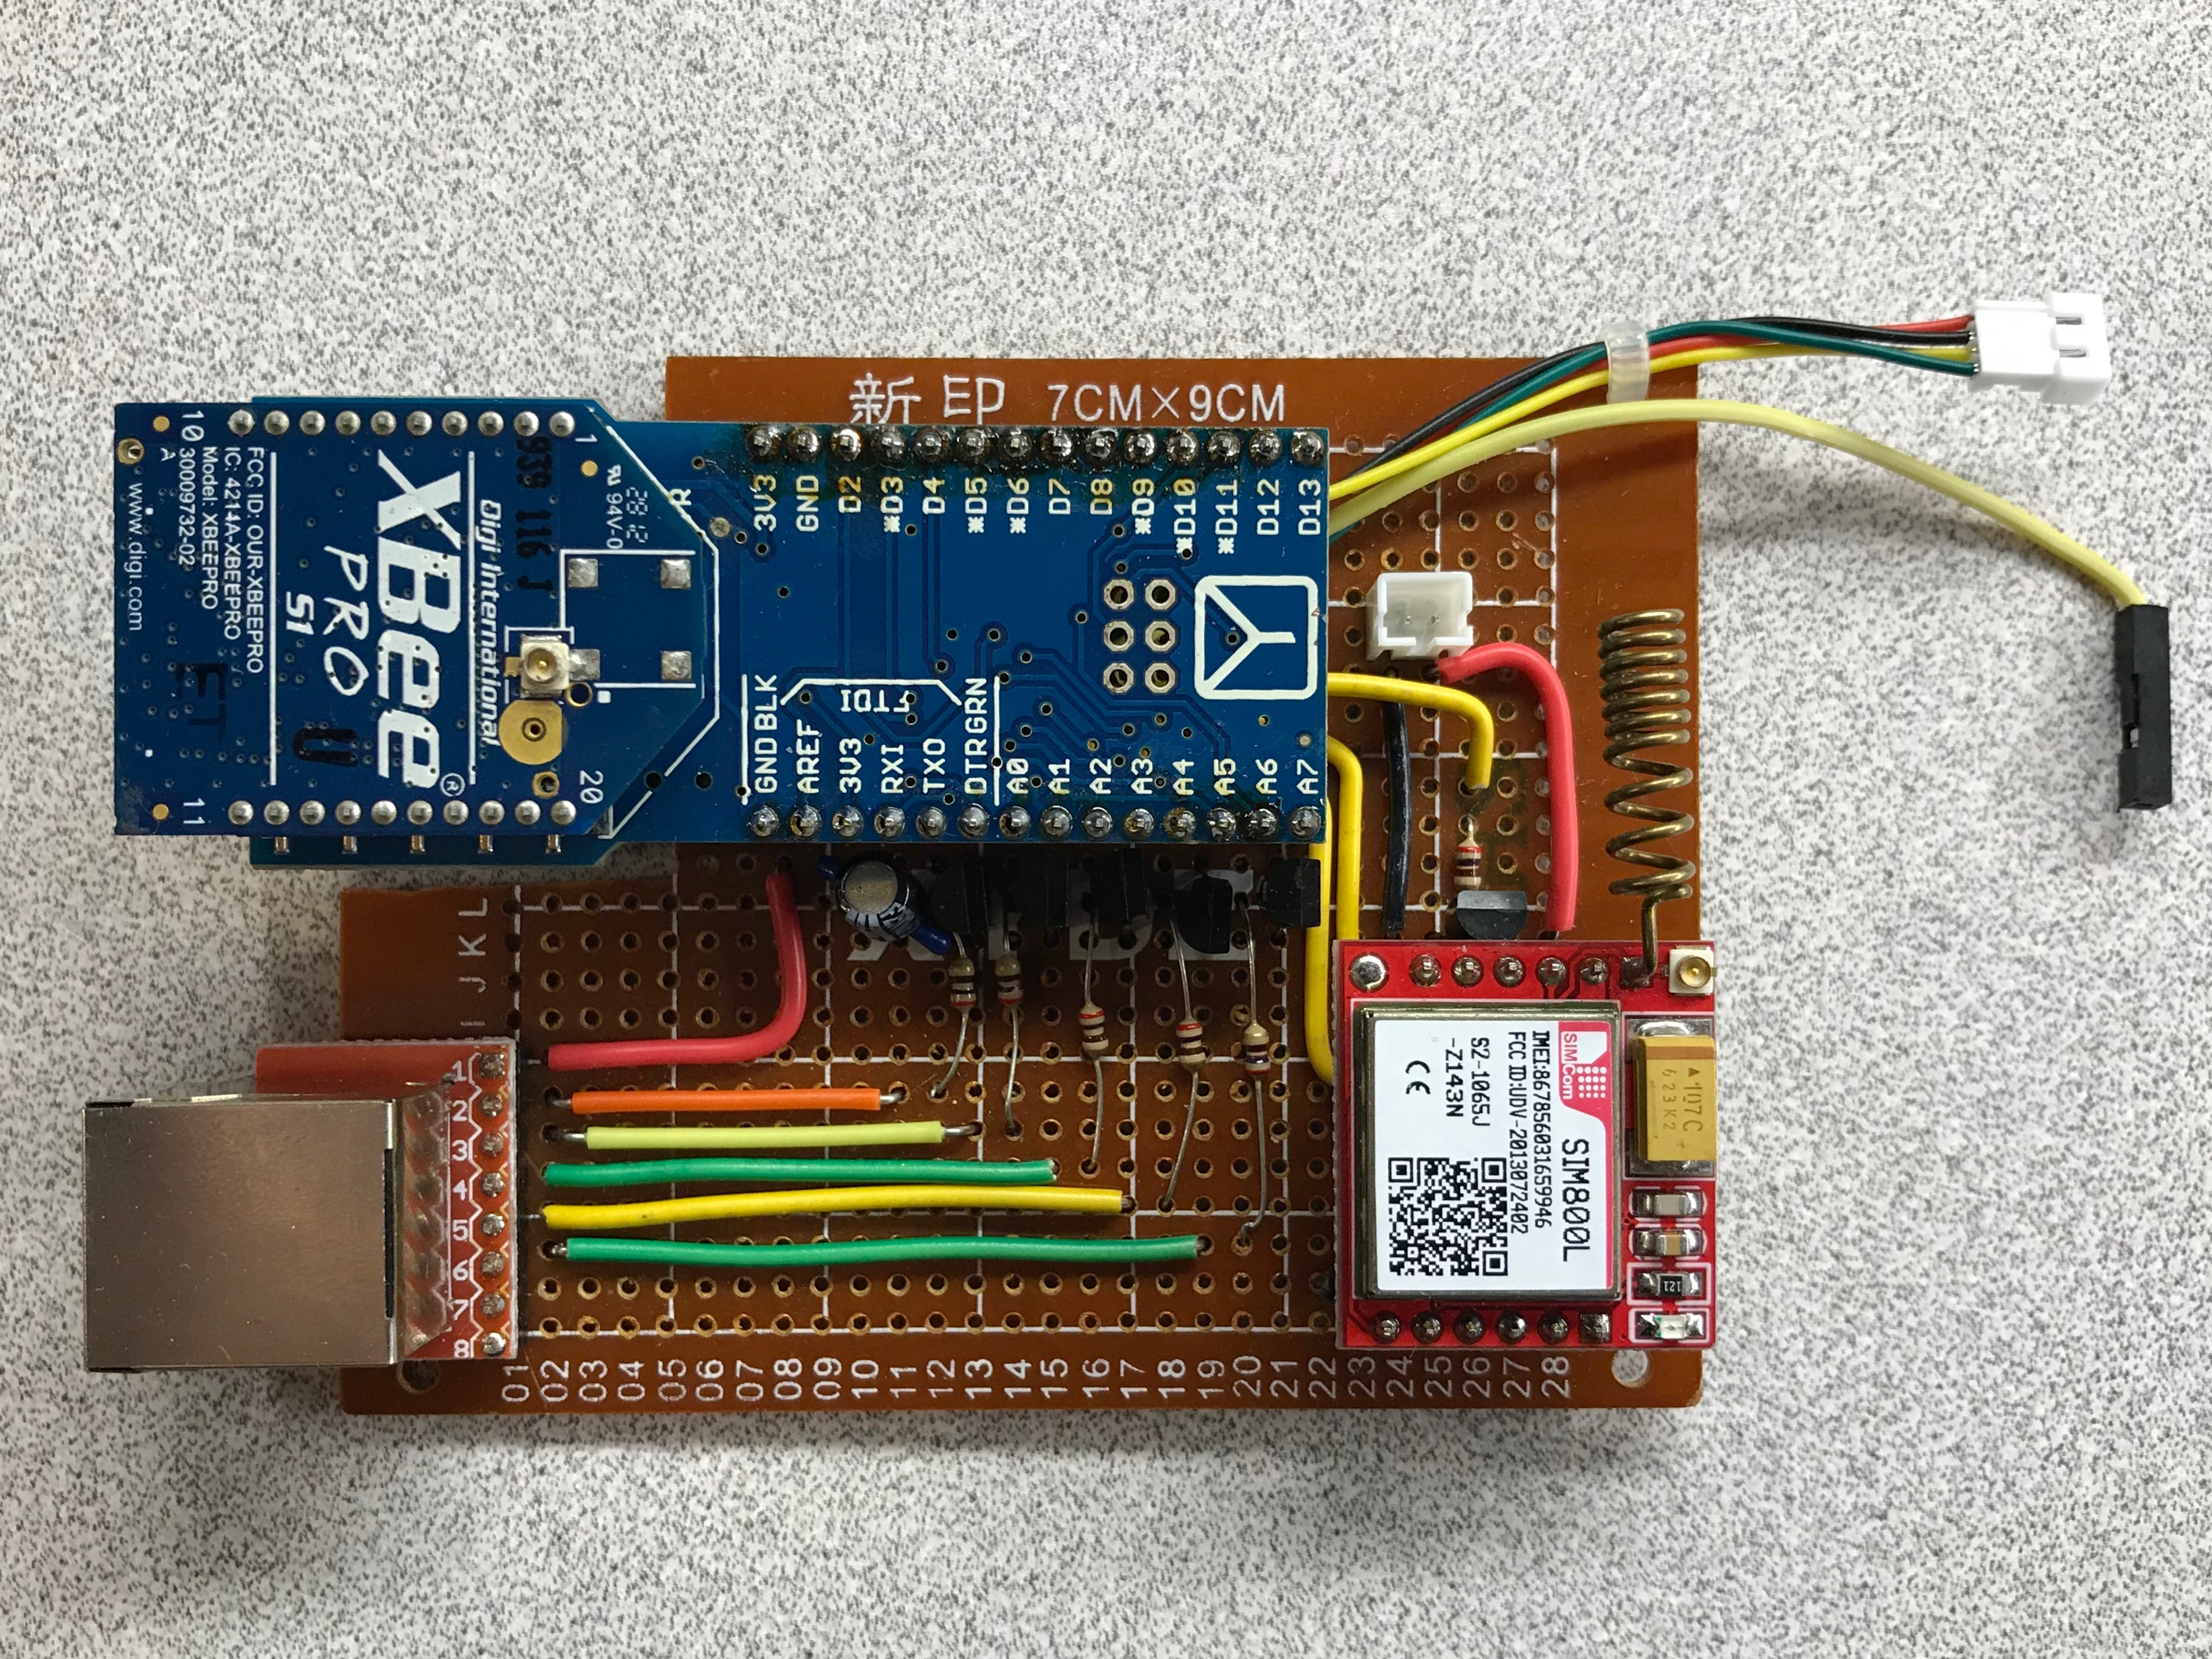
\includegraphics[width=.7\textwidth]{img/v2_controlBoard.jpg}
	\caption{\label{fig:v2_controlBoard} This is a figure of the version 2 control board.}
\end{figure}

Version two expanded the feature set significantly, in preparation for the printed circuit board (PCB) design in version 3 of the control board. Features that I implemented in the second version of the control board include: wireless programming, a roadway temperature sensor, and solar charging. In addition to the new operational features, there was significant technical optimization regarding power consumption, the battery and charge system, water sensor improvements, and communication improvements. 

\paragraph{Wireless programming} In the actual implementation of this type of device, it is important to be able to rapidly transfer new software to the deployed units. Rather than having to go to the physical main board on the deployed unit, I decided to prototype wireless programming with my initial design. With this feature, an individual can go within a close proximity to a unit and re-flash the software on it without having to remove the unit. This feature currently works for one unit; however, I would like to explore the possibility of programming the entire network of devices at once. This could come to fruition through adjusting EEPROM memory with a HTTP pull request from my cellular module. 

\paragraph{Roadway Temperature Sensor} A second inexpensive yet useful feature that I implemented in v2 is a roadway temperature sensor. Since these units will be placed all through a city with the water sensor being close to the ground, I decided to have the option to capture roadway temperature during the winter months. This increases the utility of the DROP sensor as it is capable of providing useful data year-round with this temperature probe. A waterproof probe will be placed along the ground to give an estimation for icing conditions. If parts of the city face lower/higher roadway temperatures due to sun exposure or other features of the earth, they should be treated first for ice. This only increases the per unit cost of drop ~\$3, so whilst it is not the primary feature of DROP, it is worth adding. This feature is something I learned would be useful from my calls to city engineers in the midwest. 

\paragraph{Solar Charging} The initial plan was to develop a power harness that was easy to integrate with existing city power infrastructure found in stop lights and streetlights. I was able to optimize the power consumption of the circuit, so I opted to change to a solar powered system instead of ``shore power''. This aids in ease of implementation and fail-safe design during a natural disaster. I designed and printed a housing for a solar panel of adequate size. See figure \ref{fig:3dPrintHousing}.

\begin{figure}[ht]
	\centering
	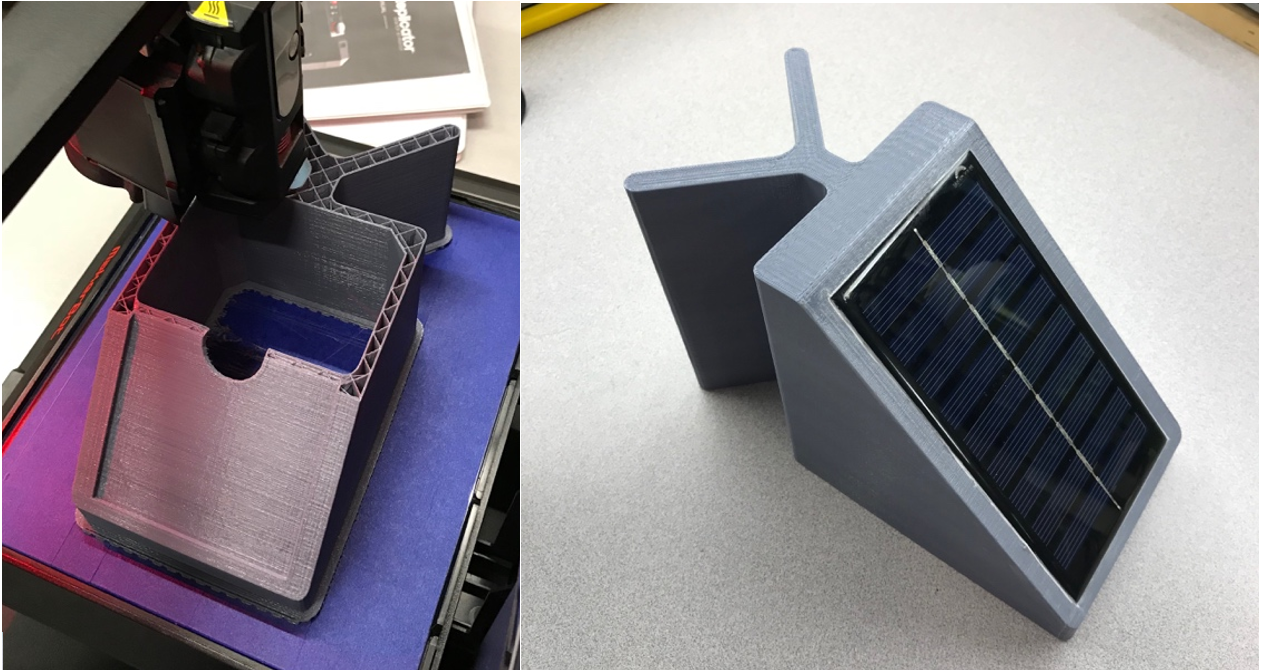
\includegraphics[width=.8\textwidth]{img/3dPrintHousing.PNG}
	\caption{\label{fig:3dPrintHousing} This figure the 3d printed housing with an inline solar panel.}
\end{figure}

From my calls with city engineers, I learned that ease of implementation is of paramount importance. To make these units easy to install, I created a housing with a Y shaped mounting point. This version of the housing will be very easy to mount on tubular objects. A large metal hose clamp can be assembled around the base of the Y shaped housing (in a slot that I left) to easily affix the control board housing to a street-light pole, telephone pole, or a stop light. 

\paragraph{Power Consumption} In order to have a successful long-term deployment of the DROP sensor, it is necessary to have a very low standby current of the control board. When the sensor is disabled, it is necessary that the power consumption of the circuit minimized so the battery charging current from the solar panel can be at a maximum. To achieve this, I needed to optimize each part of the sensor. The parts of the main board that can be optimized for power consumption are the Atmega 328p IC (the main microcontroller), the XBee (wireless short-range radio), and the SIM800l (the cellular communication module). The passive components in the circuit, such as pullup resistors and the transistors draw very little current and there was little room or need for optimization. 

\subparagraph{ATMEGA 328p Integrated Circuit} The power draw of this component was fairly low to begin with, drawing 6.5mA. However, I did research online and found an Arduino library that allows for a sleep mode. The sleep mode can be user defined to wake with an interrupt pin or on a timer. The interrupt pin functionality works very well for DROP because the first level of my water sensor can be used as the interrupt pin, signaling to wake the device. As soon as water reaches a certain level, it will wake the circuit and begin to transmit data. Once I programmed the Arduino to enter into sleep mode, the power consumption was dramatically reduced. The Atmega328 now draws 30uA, equating to a power reduction of over 200x when it is in sleep mode. 

\subparagraph{XBee} The XBee is a short-range wireless radio that can be used to create point to point and mesh networks. The one downfall is that it consumes a fair amount of power when it transmits and when it is on standby. I conducted an initial test to determine the peak and standby power consumption of the device (as this is an important factor for designing my power regulation circuit). To measure this, I set up a 1 $\Omega$ shunt resistor in series and measured the voltage drop with my oscilloscope (shown in Figure \ref{fig:powerDraw}). Peak power under transmission for the XBee and an Atmega 328p is 350mA and standby current was 70mA. In comparison to the Atmega 328p (the microcontroller) this wireless radio consumed significantly more power when operating (14x more than Atmega 328). To reduce this value, I researched sleep modes for the XBee radio. I found a few different sleep modes in the documents for the radio and I programmed the radio, designating one of the I/O pins to be a sleep toggle pin. Now, the microcontroller can enable or disable the sleep state of the XBee radio. When the XBee radio is disabled, it draws approximately 300uA. When in the sleep-state, the XBee draws over 230x less power. 

\begin{figure}[ht]
	\centering
	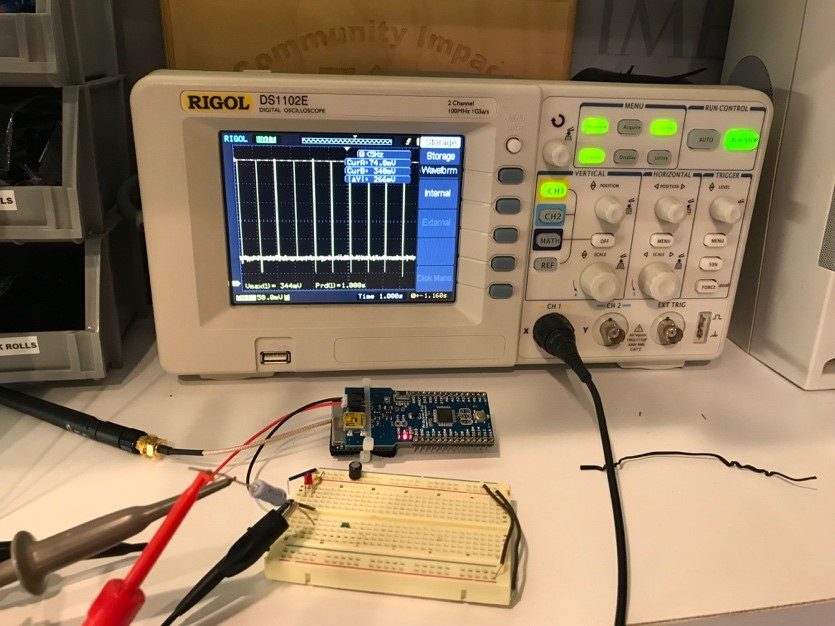
\includegraphics[width=.5\textwidth]{img/powerDraw.jpg}
	\caption{\label{fig:powerDraw} This figure shows the power draw of the xBee Transmitter.}
\end{figure}

\subparagraph{SIM800L} The SIM800L is the cellular module for the system. It is similar to the chipset found in a standard cell phone. To make this operational, I have a SIM card that I place in the circuit. It has an attached phone number. The cellular radio draws a fair amount of power, requiring nearly 2A at peak transmit power. However, issuing a sleep command from the microcontroller in DROP v2 can reduce the sleep power to less than 1mA. While this is the most power hungry device, careful moderation of sensor updates and the sleep mode still allows cellular communication to be a viable option for long term data transmission.  

\subparagraph{V2 Total Power Consumption Testing} In a sleep state, the entire circuit draws ~2mA, which is more than adequate for this sensor. The passive resistors, transistors, and loss due to the voltage regulation account for very small contributions to total current consumption. 

\paragraph{Battery Charge and Discharge System Design} The reason I have conducted such deliberate power consumption testing is to optimize charge time for the battery during a natural disaster. I want the ability to customize sensor update frequency, or power up different parts of the module for differing needs. I want the sensor to operate for the longest period of time with the quickest update rate. Version two uses an 18650 LiPo battery to power the circuit. I choose this battery because of its easy-to-implement and easy-to-replace form factor. The battery is shown in figure \ref{fig:batteryHolder}

\begin{figure}[ht]
	\centering
	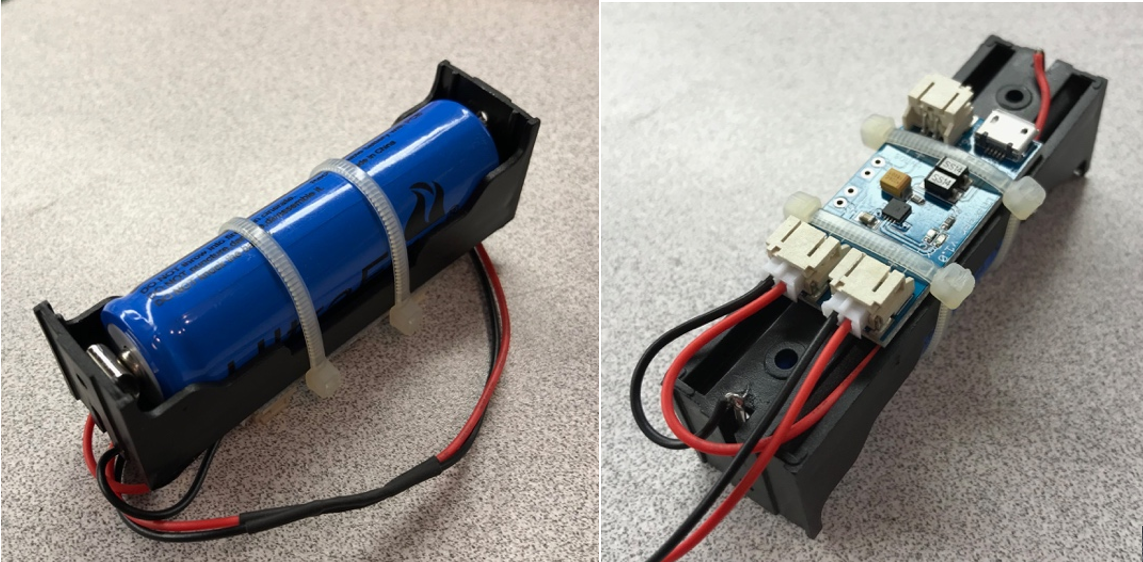
\includegraphics[width=.7\textwidth]{img/batteryHolder.png}
	\caption{\label{fig:batteryHolder} This figure shows the 18650 battery and solar charger.}
\end{figure}

It sits in a battery holder and is easily repairable. In addition, it is fairly inexpensive for its size. It is a 2500mAh battery and costs \$2 for an off-brand option on eBay. The batteries on reputable electronics parts distributors cost a little more, but there are reasonable price breaks for large enough quantities, making this battery option viable for mass manufacturing. Regardless, it is a ubiquitous battery size that should power the circuit for a decent period of time. In a flood circumstance, I plan for the circuit to power on, update the readings, then sleep for ~30s then update again.

In full sunlight the solar panel will produce anywhere from 100-250mA. This will charge the battery over the course of two days from a completely discharged state while the main board is in a sleep state. I am using a drop-in MPPT solar charger that maximizes the power output of the solar panel by adjusting the voltage at which it operates at. This will ensure the panel is being optimized for maximum power output. 

\paragraph{Communication Design} As I described above, Version 2 implements two independent radios. The data can either be transmitted via XBee or be pushed to an online webserver/sent via SMS with the cellular unit. The SIM800L cellular unit is currently programmed to send SMS alerts to my phone for each change in water depth. One neat feature of the XBee radios is the functionality for a mesh network - with this ability, if the sensors are placed in a dense enough area they can form a mesh network where I could capture all the data in a city with one base station. Currently, I am using a series 1 XBee radio which I can use for wireless programming and data transmission, but it does not support the mesh networking. Both the series 1 and series 2 have the same pinout, however, so it should be a drop in replacement if I ever choose to want mesh networking. 

\subsection{DROP Control Board Version 3}
As I beta tested many new features in v2 of the control board, I finalized the designs and implemented them into the final revision of the DROP control board in version 3. The creation of a dedicated PCB for the control circuit will help in the mass manufacturing of this device. In the following two pages, I have included a schematic drawing and board rendering of the final DROP circuit. Considering this is a physics honors project centered around electrical circuit design, the design process and final outcome of this circuit is my most novel single outcome. The development of this step was much more intensive than I initially expected. In addition to translating my V2 board into a schematic, I also had to source the components to populate this board and source the `footprints’ for the actual various components. I ended up simplifying my design with resistor arrays and transistor arrays to fit more components in a smaller area.


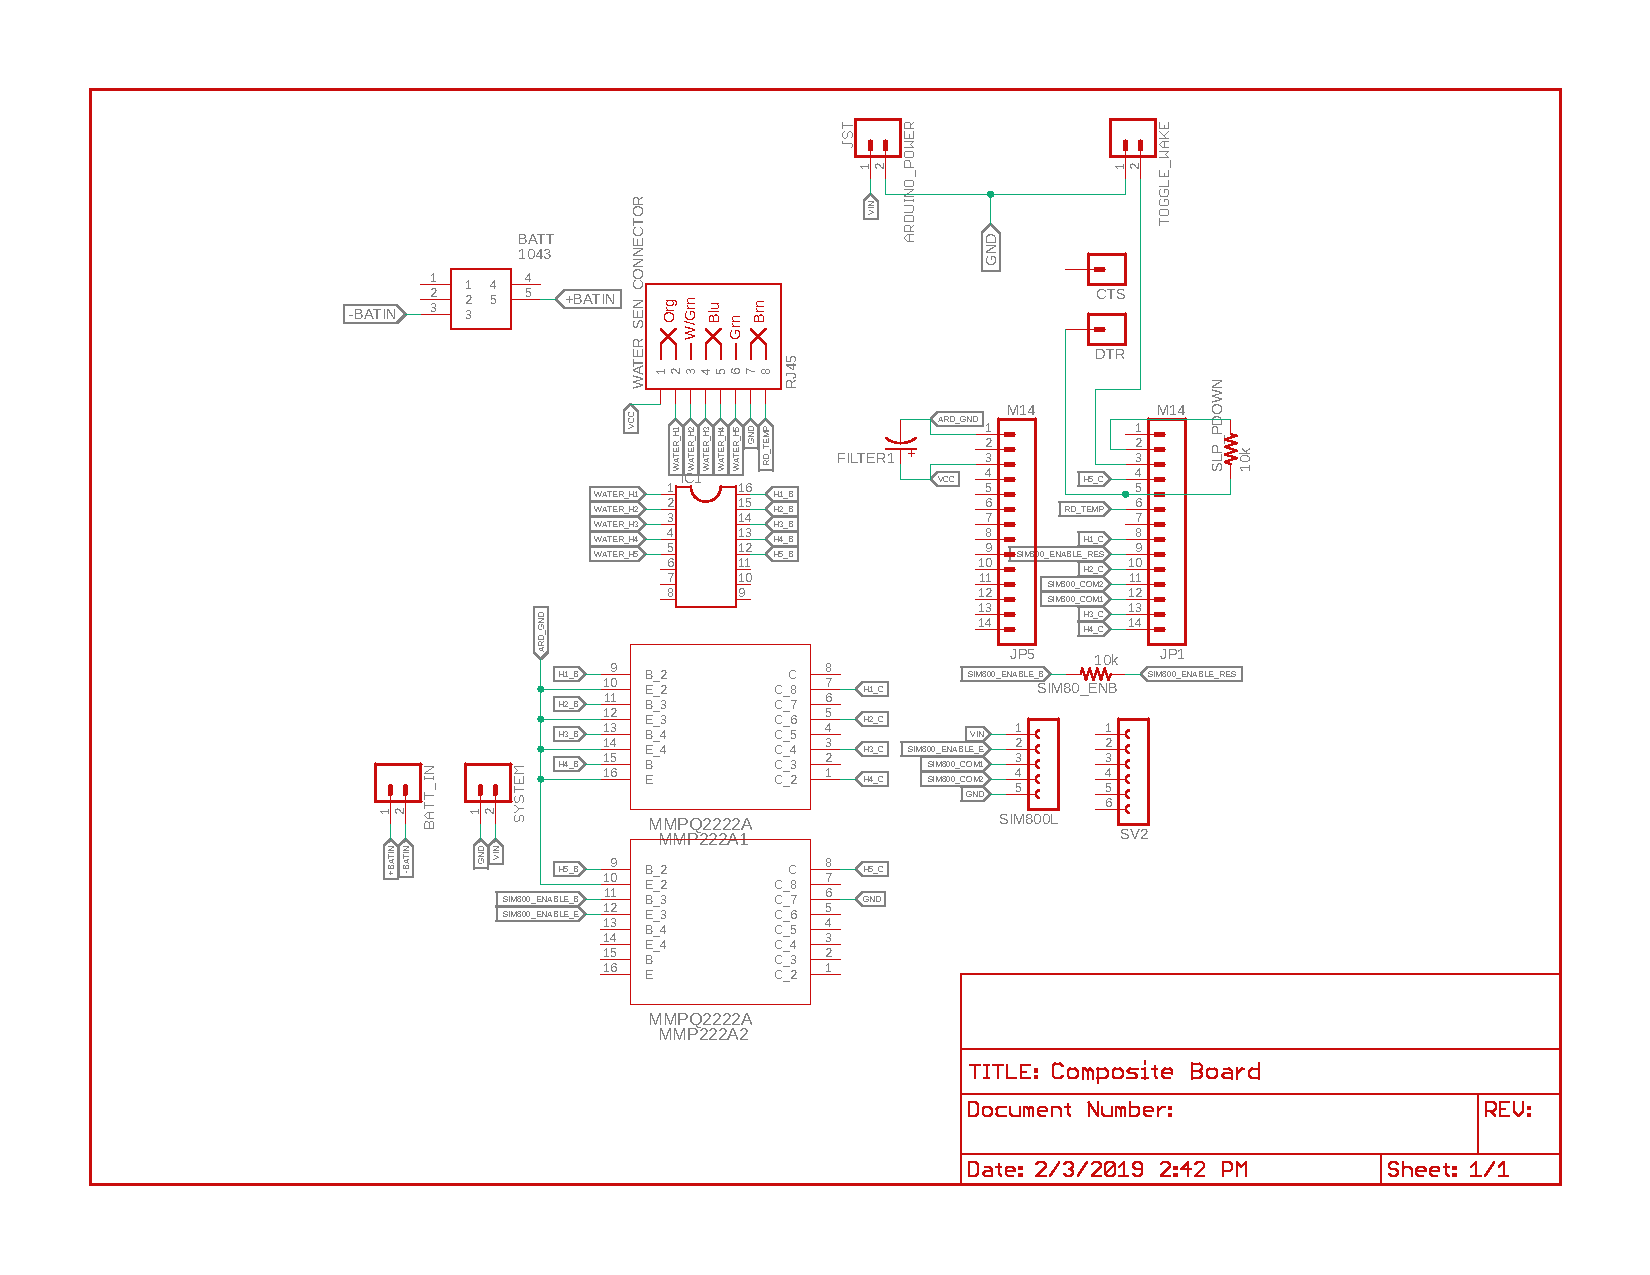
\includepdf{img/CompositeSchematic.pdf}
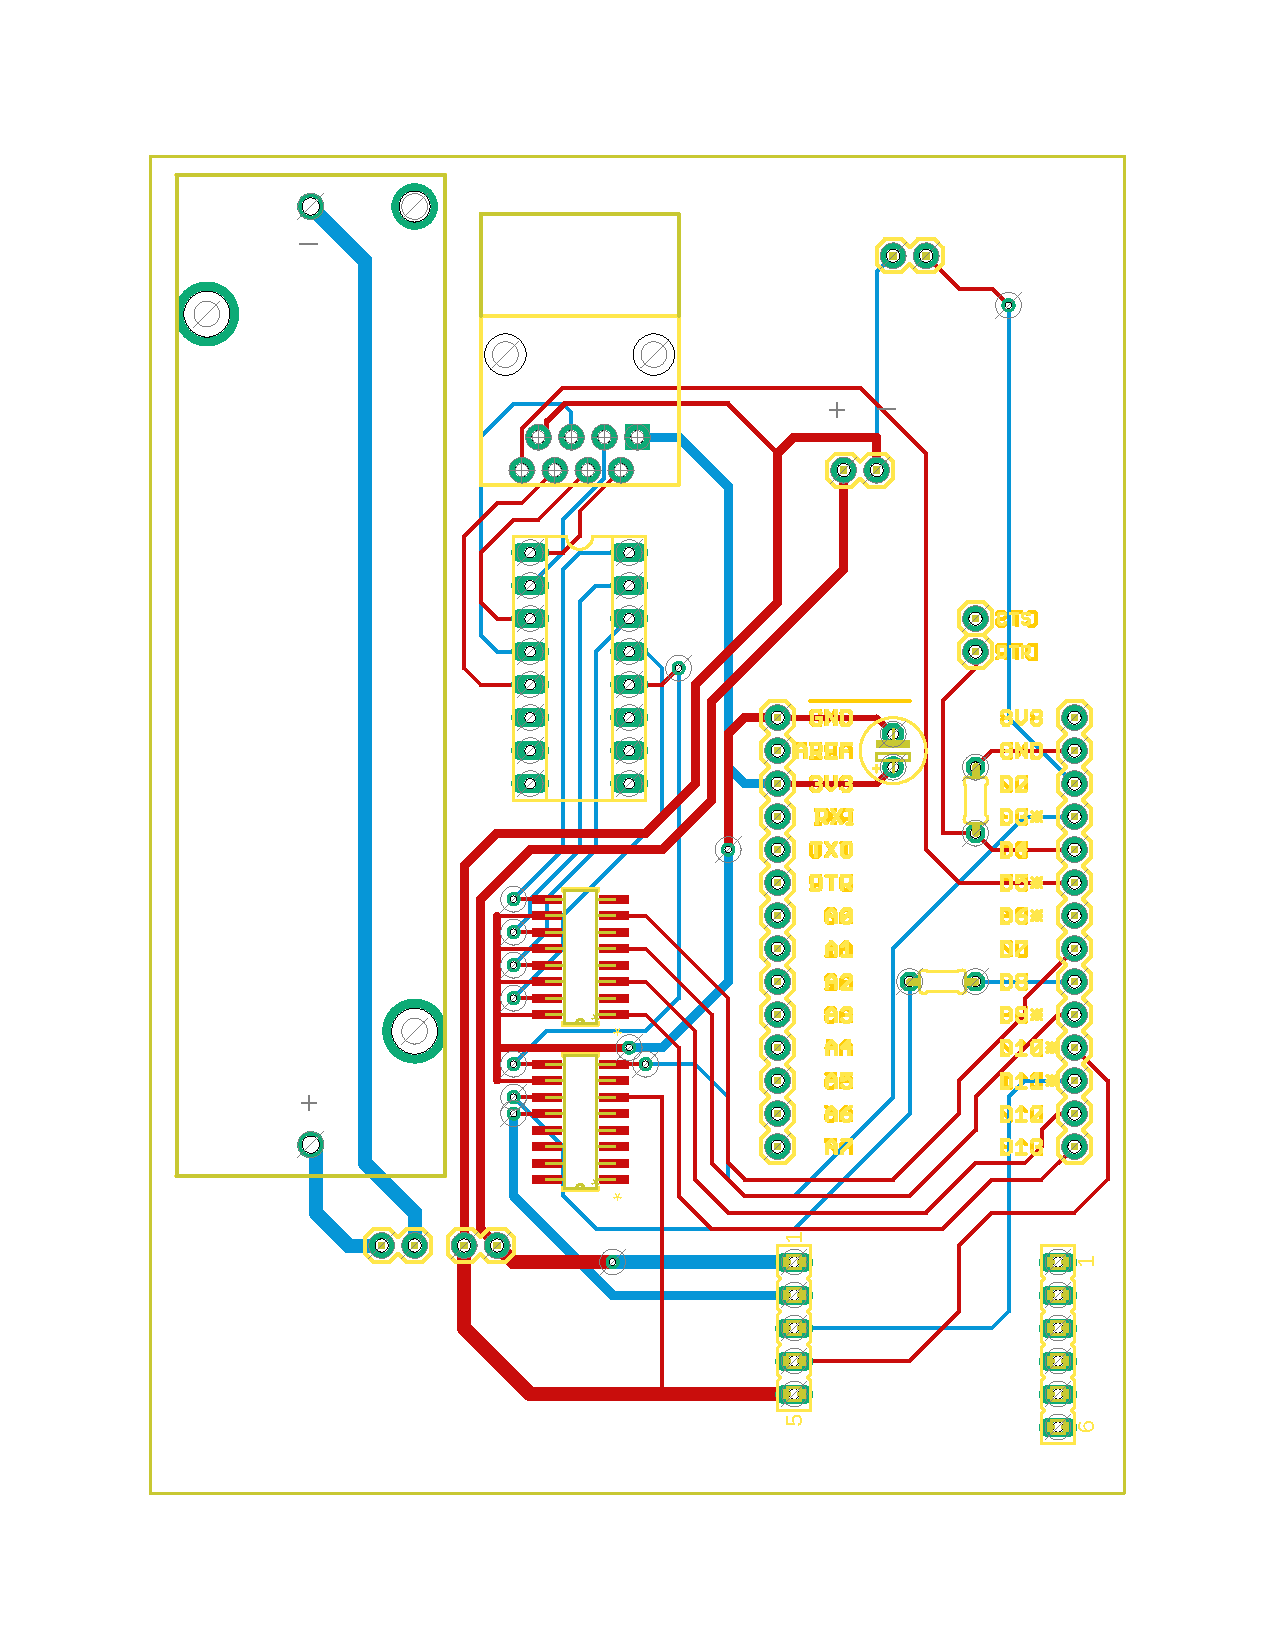
\includepdf{img/CompositeBoard.pdf}


\section{Water Sensor Design}
The water sensor works in conjunction with the control board, providing an electrode framework to sense the water level. This section involves the problem solving process to make a visually appealing, durable, and scalable design.

\subsection{Ideation and Initial Prototype} When designing a device for a flood, the method for capturing water depth must be very robust. Flood scenarios often consist of heavy rain, with quickly moving flood waters containing silt and debris. An appropriate flood sensor must accommodate all of these factors. An initial method I thought about to measure water depth was a distance sensor mounted on the control board on an elevated surface. As flood waters rose, the distance sensor would report a shorter distance. I dismissed this idea because of the potential for wildly inaccurate readings with shrubbery, debris, and rain to interfere. Another way to measure water depth is with a pressure sensor. This is often used for depth readings in tanks. While accurate for still fluids, this would not work with silt and changing pressure in a moving flood water. The final design I settled on capitalizes on the slight conductivity of water. It uses an electrode based sensor with transistor amplifiers to measure discrete water levels. This should be immune to quick flowing waters, and resistant to silt and debris in the water. To test this, I developed a very rudimetry prototype. The first prototype was constructed with a few wires as the electrodes and hot glue to attach them to a board. While it was functional and showed proof of concept, it was not robust for a true flood scenario. 

\subsection{Water Sensor Version 2} With the second prototype, I wanted a highly customizable model to test various electrical and mechanical configurations. To do this, I 3D printed a bracket that would hold wires in place within a PVC pipe. I used a very commonplace CAT5 wire and I stripped it to the correct lengths. With this sensor, I also tested an RJ45 connector to link the water sensor to the control board. I choose this connector (and ended up implementing it in version 3) because it is very inexpensive and easy to manufacture. This sensor and connector design functioned properly, and it was highly customizable for testing. The 3D printed brackets were friction fit into place, allowing the user to customize the termination point for each wire. The termination point of the wire translates to the discrete levels the flood water will be measured at. However, this sensor design would not be easy to mass manufacture, and the sensor was not particularly sleek.

\begin{figure}[ht]
	\centering
	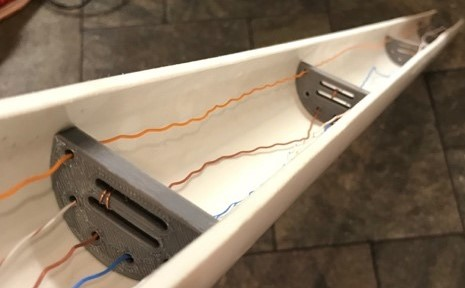
\includegraphics[width=.6\textwidth]{img/v2_waterSensor.jpg}
	\caption{\label{fig:v2_waterSensor} This figure shows the version 2 of the water sensor, featuring a 3d printed clip-in electrode bracket.}
\end{figure}

\subsection{Water Sensor Version 3}
For the third revision of the water sensor, I worked to create a design that was more visually appealing and was easy to mass manufacture. To do this, I designed a printed circuit board that will be mounted in an aluminum housing. Figure \ref{fig:v3_waterSensor} is one of the design files for the circuit board.

\begin{figure}[ht]
	\centering
	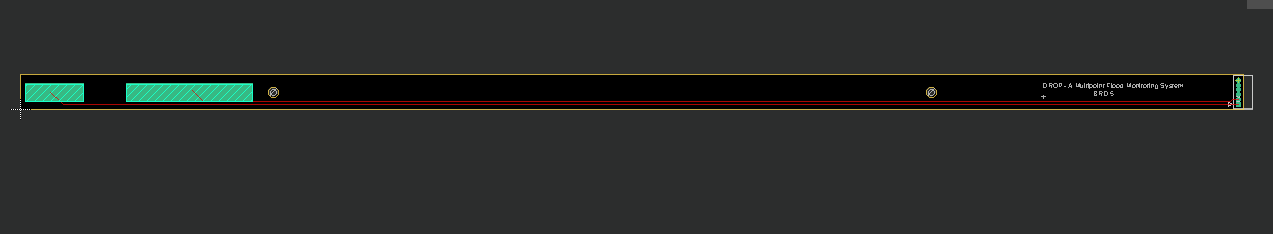
\includegraphics[width=1\textwidth]{img/v3_waterSensor.png}
	\caption{\label{fig:v3_waterSensor} This figure shows the design file for the third version of the water sensor electrodes.}
\end{figure}

 I sent the design files to a PCB manufacturing service and had a few units created. Figure \ref{fig:v3_waterSensorCollage} is an image of the final product. With this design, the sensor looks much more professional in a smaller form factor. It will look even more sleek when deployed on a streetlight/light post. The aluminum housing should blend in nicely for a visually appealing result. It is only 1.6cm wide and 0.7cm thick. It is 2m long (~6.5ft). However, I designed the circuit boards in a way that the sensor can be extended or shortened to any desired length (thus increasing the range of water depth measurement). The modular design of the boards allows for a wide range of applications outside of urban flood monitoring. The same sensor could be used for stream and river depth monitoring or crop field flood monitoring. 

\begin{figure}[ht]
	\centering
	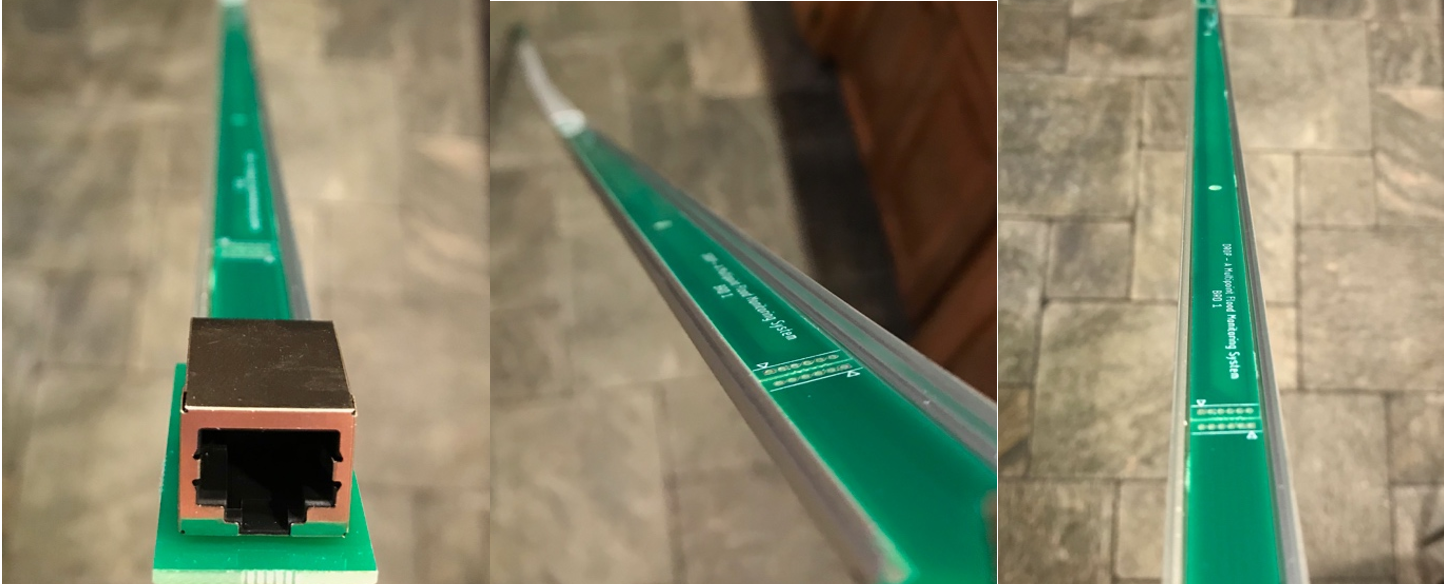
\includegraphics[width=1\textwidth]{img/v3_waterSensorCollage.png}
	\caption{\label{fig:v3_waterSensorCollage} This figure shows the final water sensor, mounted in an extruded aluminum channel.}
\end{figure}

\section{Current State and Future Plans}

The current DROP flood monitoring system is utilizing the third generation control board and the third generation water sensor. When I set out to work on this honors project, I aimed to create an open-source, easy to manufacture, and easy to implement flood monitoring system. Through my iterative design process, I believe I have achieved these goals. The manufacturing processes I used are easy to scale. The bulk of the control board is manufactured with a PCB and SMD/PTH components. A production run of many of these units is very feasible. In the event of a component failure, most components are cheap and easy to replace with my modular design of the board. The housing for the flood monitoring system is currently 3d printed. For mass manufacturing, this would have to be translated to an injected mold or something similar. Additionally, the water sensor is built using a PCB based electrode. In addition to the ability to scale PCB production, the design is very modular, making it easy to change the length of the water sensor for a multitude of applications. Finally, I believe the feature set I implemented will be robust for easy implementation. Options such as wireless programming allow technicians to easily change the software on the devices without having to physically interact with the devices. Given that most of the monitors will be mounted in high locations (to avoid flood water), this feature will be particularly handy for ease of updating software. In addition, I opted to use solar power to create an environmentally friendly and easy-to-install solution. Rather than relying on any form of grid power or having to find power, I optimized the power consumption of all the components to fit within the constraints of a solar powered device. Finally, the cellular communication feature will be very useful to create a network of these internet-of-things devices, all pushing data to an online webserver. These design features make a final product that is relatively inexpensive, easy to manufacture, and easy to implement. 

Moving forward, I plan to publish the finished design files for the maker community to learn from and critique. I have been ideating about how to run a pilot program to test the utility of DROP. Currently, I think the best way to field test a device like DROP is to create a small batch of test units (10-15). When a storm system is predicted to hit a certain area, the test units can be quickly deployed to that area. I believe this is one of the most cost effective ways to run a pilot program and begin generating test data to show the utility of this device in the event of a storm system. If the opportunity presents itself, I hope to continue pursuing this project.  

I am very proud of the progress I have made over the past year. This educational process has contributed to a very pratical and engineering-based side to my physics major. I have been able to identify and refine a problem through market research, and design a solution that uniquely solves the identified problem. I would like to thank Dr. Baker for his guidance throughout this process, making the development of this sensor possible. 

\pagebreak
\begin{thebibliography}{9}
\bibitem{floodDeaths}
	Lam, Linda. “A Concerning Trend: Flooding Deaths Have Increased in the U.S. the Last Few Years.” Weather.Com, The Weather Channel, 8 Nov. 2018, weather.com/safety/floods/news/2018-11-08-flood-related-deaths-increasing-in-united-states.
\bibitem{economicImpact}
	Amadeo, Kimberly. Floods' Effect on the Economy and You. The Balance, 2 Feb. 2019, www.thebalance.com/mississippi-river-flooding-3305663.
\bibitem{floodDays}
	Upton, John. Warming Brings Increasing Flood Risk And Heavier Rain. Climate Central, 7 Mar. 2016, www.climatecentral.org/news/warming-increasing-flood-risk-heavier-rain-20108.

\end{thebibliography}
\end{document}